\label{sec:intro}

La utilización de imágenes satelitales permite analizar grandes extensiones del
territorio, contando con un registro histórico con el cual realizar
comparaciones.

En la provincia de Misiones, el departamento de Iguaz\'u es lindante a Brasil y
Paraguay siendo parte de la zona conocida como triple frontera
perteneciente a la ecorregi\'on conocida como \emph{selva paranaense} (Figura \ref{parque}). Dentro
del mismo podemos encontrar la Represa de Urugua-\'{\i} y el Parque Nacional
Iguaz\'u. El departamento tiene un area de $2.736 km^2$ y una poblaci\'on de
$82.227$ seg\'un el \'u;timo senso del INDEC.

\begin{figure}[h!]
  \centering
  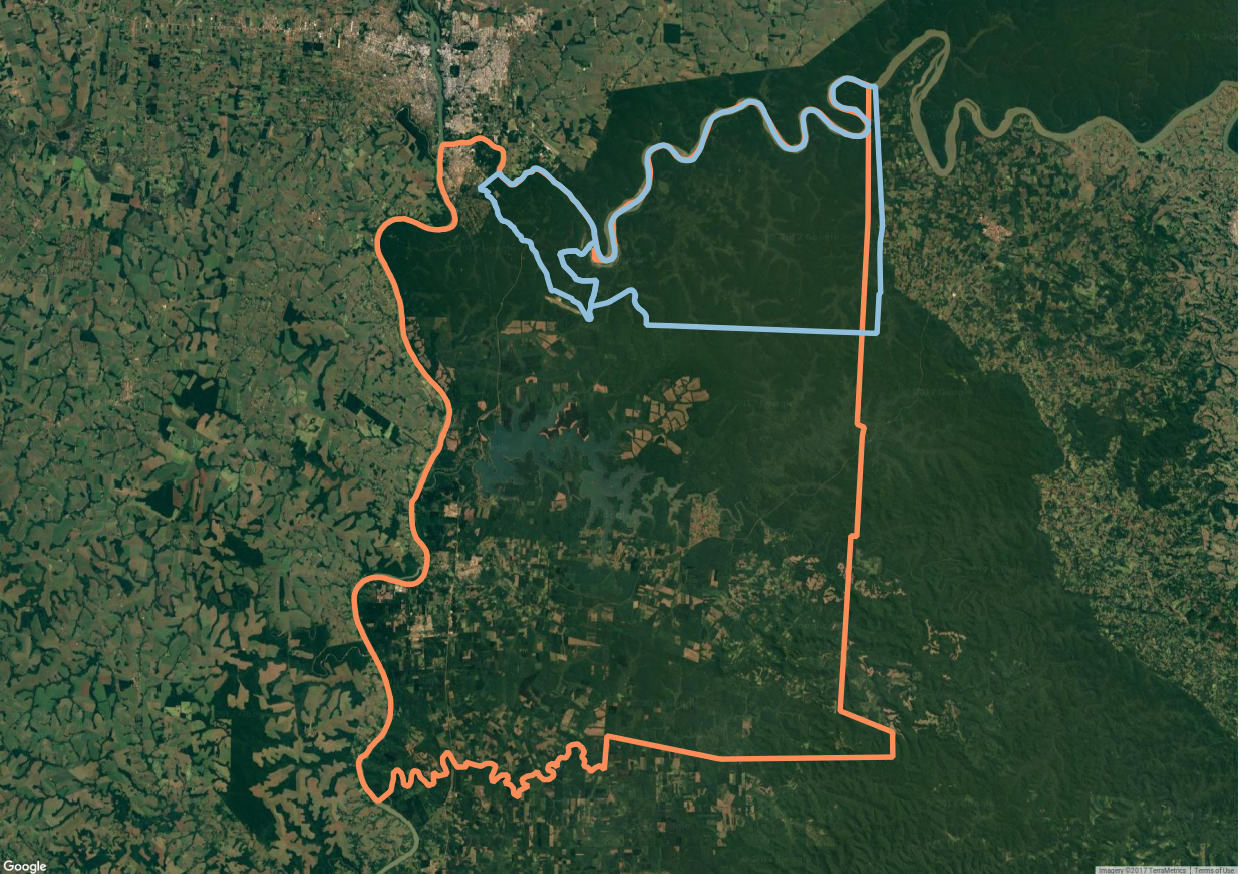
\includegraphics[width=0.8\textwidth]{triple.png}
  \caption{Departamento de Iguaz\'u, en rosa, y parque natural Iguaz\'u, en celeste.}
  \label{parque}
\end{figure}

Tomaremos entonces al departamento como \'area de estudio durante este curso
con el objetivo de obtener un mapa de uso y cobertura dentro del mismo que nos
permita estimar y validar  las \'areas correspondients a los mismos.

Utilizaremos para esto imagenes satelitales de los satelites Landsat 8, Landsat 7 y
el producto de MOD13Q1 obtenido de los satelites TERRA y AQUA obtenidas durante
el periodo 2000-2016.

\section{Organizacion del curso}

El curso se divide en dos partes. En la primera trabajaremos con la compresion
del espacio espectral y el uso de las imagenes satelitales para extraer valores
continuos de las variables biofisicas.

En el capitulo \ref{viaje}, \nameref{viaje}, estudiaremos la firma espectral de
distintas coberturas, veremos como se relacionan con las propiedades biofisicas
de ellas y por ultimo introduciremos el concepto de espacio espectral como el
lugar natural donde realizar el analisis en teledeteccion.

En el capitulo \ref{rebotando}, \nameref{rebotando}, estudiaremos distintas
formas de obtener la reflectancia de las coberturas a partir de los datos obtenidos
por un satelite. En el estudiaremos metodos de correccion atmosferica basados
en propiedades estadisticas de las imagenes y en el modelado de la atmosfera.

En el capitulo \ref{abaco}, \nameref{abaco}, veremos como a partir de los valores
de reflectancia para una cobertura y operaciones matematicas entre los mismos,
podemos obtener los valores de variables biofisicas continuass como pueden ser
el contenido de clorofila o humedad.

En la segunda parte del curso vamos a trabajar mas en detalle con el espacio
espectral y vamos a usar sus propiedades para extraer informacion categorica de
las imagenes.

En el capitulo \ref{rotaciones}, \nameref{rotaciones}, veremos como utilizar
herramientas geometricas en el espacio de reflectancias para resaltar distintas
propiedades de las imagenes y poner en evidencia cuales son las zonas del espectro
que mas informacion aportan sobre nuesta zona de interes. Comenzaremos en este
capitulo tambien a analizar el contexto temporal para nuestras imagenes.

En el capitulo \ref{otrolado}, \nameref{otrolado}, veremos como utilizar herramientas
que no requieren de conocimiento previo del area de estudio para realizar segmentaciones
en el espacio de fases de la imagen, que luego podremos utilizar para obtener mapas
de uso y cobertura. Comenzaremos en este capitulo tambiena analizar el contexto
espacial de cada pixel.

En el capitulo \ref{educando}, \nameref{educando}, veremos otros metodos para extraer
informacion categorica sobre las imagenes satelitales al estudiar distintas
formas de clasificacion supervisada. Comenzaremos en este capitulo tambien a
analizar mas en detalle cuales son las coberturas que mayores problemas generan al
momento de realizar clasificaciones

En el capitulo \ref{pos}, \nameref{pos}, veremos algunas tecnicas de postprocesamiento
que nos permitiran analizar el contexto espacial de nuestras clasificaciones y
comenzar a calcular areas de cobertura para nuestras imagenes con su correspondiente incerteza.

\subsection{Cronograma}

Duranto el curso trabajaremos con el siguiente cronograma

\begin{itemize}
  \item[25/4] Instalar el QGIS y el R. Ver apendice.
  \item[26/4] \nameref{viaje}
  \begin{itemize}
    \item Clase teorica: radiancia y reflectancia. Firmas espectrales y espacio espectral.
    \item Clase practica: capitulo \ref{viaje} de la guida practica.
    \item Lectura recomendada: Remote sensing digital Image Analysis - Jogn A. Richards. Capitulos 1 y 3
  \end{itemize}
  \item[2/5] Entrega del cuestionario 1.
  \item[3/5] \nameref{rebotando}
  \begin{itemize}
    \item Clase teorica: Transferencia radiativa. Metodos estadisticos y modelado de la atmosfera.
    \item Clase practica: capitulo de \ref{rebotando} la guia practica.
    \item Lectura recomendada: Remote sensing digital Image Analysis - Jogn A. Richards. Capitulos 2
  \end{itemize}
  \item[9/5] Entrega del cuestionario 2.
  \item[10/5] \nameref{abaco}
  \begin{itemize}
    \item Clase teorica: C\'alculo de indices espectrales
    \item Clase practica: capitulo de \ref{abaco} la guia practica.
    \item Lectura recomendada: Quantitative Remote Sensing - ShunLin Liang. Capitulos 8
  \end{itemize}
  \item[16/5] Entrega del cuestionario 3.
  \item[17/5] Clase de consulta.
  \item[23/5] Entrega del trabajo practico 1.
  \item[24/5] \nameref{rotaciones}
  \begin{itemize}
    \item Clase teorica: Transformada Tasseled Cap y Analisis por componentes principales.
    \item Clase practica: capitulo de \ref{rotaciones} la guia practica.
    \item Lectura recomendada: Remote sensing digital Image Analysis - Jogn A. Richards. Capitulos 6
  \end{itemize}
  \item[30/5] Entrega del cuestionario 4.
  \item[31/5] \nameref{otrolado}
  \begin{itemize}
    \item Clase teorica: Metodos de clasificacion no supervisados.
    \item Clase practica: capitulo de \ref{otrolado} la guia practica.
    \item Lectura recomendada: Remote sensing digital Image Analysis - Jogn A. Richards. Capitulos 9
  \end{itemize}
  \item[6/6] Entrega del cuestionario 5.
  \item[7/6] \nameref{educando}
  \begin{itemize}
    \item Clase teorica: Metodos de clasificacion supervisados.
    \item Clase practica: capitulo de \ref{educando} la guia practica.
    \item Lectura recomendada: Remote sensing digital Image Analysis - Jogn A. Richards. Capitulos 8
  \end{itemize}
  \item[13/6] Entrega del cuestionario 6.
  \item[14/6] \nameref{pos}
  \begin{itemize}
    \item Clase teorica: Tecnicas post clasificacion.
    \item Clase practica: capitulo de \ref{pos} la guia practica.
    \item Lectura recomendada: Making better use of accuracy data in land change studies: Estimating accuracy and
area and quantifying uncertainty using stratified estimation - Olofsson et al.
  \end{itemize}
  \item[20/6] Entrega del cuestionario 7.
  \item[21/6] Clase de consulta. Arreglar horario.
  \item[27/6] Entrega del trabajo practico 2.
  \item[30/6] Entrega de certificados.
\end{itemize}

\subsection{Forma de aprobacion}
Para aprobar el curso se deben juntar al menos 100 puntos entre las distintas actividades.
Adem\'as se deber\'a completar un cuestionario \emph{obligatorio} sobre el curso al finalizar el mismo.

La nota final del curso estara dada por la siguiente

\begin{itemize}
\item 0 - 99 - No aprobó
\item 100-109 - Seis
\item 110-129 - Siete
\item 130-169 - Ocho
\item 170-189 - Nueve
\item 190-200 - Diez
\end{itemize}

para obtener puntos puede realizarse de la siguiente manera

\begin{itemize}
  \item Cada cuestionario: 0 a 10 puntos. Máximo 70.
  \item Cada tarea: 0 a 50 puntos. Máximo 100.
  \item Participar en la plataforma: 0 a 10 puntos. Sin máximo.
\end{itemize}

\section{Materiales del curso}
Todo el material del curso se encuentra disponible para bajar de la direccion \url{LINK DE DESCARGA}. Este se encuentra organizado de la siguiente manera

\dirtree{%
    .1 material.
    .2 aux\_data.
    .2 example\_scripts.
    .2 raster\_data.
    .2 vector\_data.
    }

conteniendo la carpeta \file{aux\_data} archivos adicionales para trabajar, \file{example\_scripts} todos los scripts que se encuentran en esta guia, \file{raster\_data} los archivos raster cada uno en una carpeta y \file{vector\_data} los archivos vectoriales para usar durante el curso.

Todos los materiales del curso, con sus correspondientes editables, pueden
encontrarse en el repositorio de github \url{https://github.com/fnemina/curso-sopi-herramientas-cuantitativas}.

En caso de encontrar cualquier problema en los materiales puede reportarlo ahi y sera subsanado en el menor tiempo posible.
